\usepackage[german]{babel}
\usepackage[utf8]{inputenc}
\usepackage{times}
\usepackage[T1]{fontenc}
\usepackage{eurosym}
\usepackage{graphicx}
\usepackage{amsmath}
\usepackage[siunitx,european]{circuitikz}
% \usepackage{ulem}
\usepackage{listings}
%
\lstset{numbers=left, numberstyle=\tiny, stepnumber=2, numbersep=5pt, language = C++, alsolanguage=XML}
% \MyLogo{\includegraphics[height=1cm]{../../../../bilder/bwslogo_3.png}}
% % \includegraphics{../../bilder/bwslogo_3.png}
% % bwslogo_3.png: 476x392 px, 300dpi, 4.03x3.32 cm, bb=
%
\only<article>{
  \usepackage[colorlinks=true,linkcolor=blue,filecolor=magenta,urlcolor=cyan]{hyperref}
}

\only<presentation>{
  \usepackage{hyperref}
}


\title{Arbeitsunterlagen zu FOS Elektrotechnik Themenfeld 12.6}
\subtitle{Elektrisches und magnetisches Feld}
\date{V 0.2.0 - im Aufbau\\ Stand: \today}%\\

\institute[BWS Hofheim]{Brühlwiesenschule, Hofheim}
\author{Thomas Maul}

\titlegraphic{Für eigene Teile gilt: \includegraphics[height=1cm]{cc_by-nc_eu.png}}

\begin{document}
  \only<article>{
    \maketitle
    \tableofcontents
    \clearpage
  }
\begin{frame}<beamer>
  \titlepage
  % \hyperlink{Teil_2}{\beamerbutton{Go part 2}}
\end{frame}
% \AtBeginSection[] % Do nothing for \section*
% {
%   \begin{frame}<beamer>
%     \frametitle{Inhalt}
%     \tableofcontents[currentsection]
%   \end{frame}
% }


% \part{Themenfeld 12.6 - Elektrisches und magnetisches Feld}
% \label{Teil_12_6}
\begin{frame}
  \partpage
  %   \tableofcontents[hidesubsections]
\end{frame}

\begin{frame}
  \partpage
\end{frame}
\begin{frame}<beamer>
  \frametitle{Inhalt}

  \begin{columns}
    \column{.5\textwidth}
    \tableofcontents[sections={7-12}]%currentsection]
    \column{.5\textwidth}
    \tableofcontents[sections={13-}]%currentsection]
  \end{columns}

\end{frame}

\section{Ladungen, Kräfte}
\only<presentation>{
  \begin{frame}{Elektronen und Atome}
    \begin{itemize}
      \item Die Materie besteht aus Atomen.
      \item Kern: Protonen und Neutronen, Hülle: Elektronen
      \item Bei Leitern: Elektronen \glq mobil\grq, bei Nichtleitern fest(er)
      \item Reibung von 2 Nichtleitern (Stoff und Glasstab)$\Rightarrow$ Ladungstrennung
    \end{itemize}
  \end{frame}
}
Die Materie besteht aus Atomen. Diese wiederum aus einem Kern mit Protonen und Neutronen und einer Hülle aus Elektronen. Bei einigen Atomen, zum Beispiel Metalle sind, ist es leicht möglich einzelne Elektronen aus der Hülle zu entfernen. Dies führt zur elektrischen Leitung - dem elektrischen Strom. Bei Stoffen, die nicht leitend sind, lassen sich die Elektronen nicht oder nur schwer aus der Hülle entfernen.

Wenn man zwei nicht leitende Gegenstände, zum Beispiel einen Glasstab und ein Stück Stoff aneinander reibt, werden durch die Reibung Elektronen in einem der beiden Gegenstände aus der Hülle herausgerissen und in die Atomhüllen der Atome des anderen Gegenstands übertragen. In diesem Moment spricht man davon, dass beide Gegenstände elektrisch geladen sind.
\begin{frame}{Katze mit Styroporflocken}
  \begin{figure}[htb]
    \includegraphics{Cat_demonstrating_static_cling_with_styrofoam_peanuts.jpeg}
    %    Cat_demonstrating_static_cling_with_styrofoam_peanuts.jpeg: 436x289 px, 180dpi, 6.15x4.08 cm, bb=
    \caption{Katze mit Styroporflocken}
    \label{abb:CatWidthStyropor}
  \end{figure}
  \footnote{Quelle: Von Original image: Sean McGrath from Saint John, NB, CanadaDerived image: Black Rainbow 999 - Diese Datei ist ein Ausschnitt aus einer anderen Datei, CC BY 2.0, https://commons.wikimedia.org/w/index.php?curid=60287175}
\end{frame}

\only<presentation>{
  \begin{frame}{Anziehung und Abstoßung von Ladungen}
    \begin{itemize}
      \item gleichnamige Ladungen stoßen sich ab.
      \item ungleichnamige Ladungen ziehen sich an.
      \item bei Elektrostatik gibt es keine Bewegung, nur Kräfte
    \end{itemize}
  \end{frame}
}

Elektrische Ladungen, die gleich sind (zwei positive Ladungen oder zwei negative) stoßen sich ab. Ladungen, die unterschiedlich sind, ziehen sich an. Die Abstoßung und Anziehung kann man als Kräfte berechnen und in gewissen Grenzen messen.

Wenn sich die Ladungen nicht zwischen den Körpern bewegen und auch nicht innerhalb des Körpers, nennt man dies einen statischen Zustand. Die Ladung ist vorhanden, die Kräfte sind vorhanden aber es gibt keine Bewegung. Unter idealen Bedingungen bleibt der Zustand dauerhaft bestehen. In der Schule vereinfachen wir. Eine Ladung ist als punktförmig definiert, sie hat keine Ausdehnung, für die Elektrostatik gilt, dass sie ohne äußere Einflüsse unverändert bleibt. Elektronen und Ladungen bewegen sich nicht.

\section[Energieerhaltung]{Energieerhaltung und Einheit}
\only<presentation>{
  \begin{frame}
    \frametitle{Inhalt}

    %  \begin{columns}
    %    \column{.5\textwidth}
    \tableofcontents%[sections={7-12},currentsection]
    %    \column{.5\textwidth}
    %    \tableofcontents[sections={13-},currentsection]
    %  \end{columns}
  \end{frame}
}

\only<presentation>{
  \begin{frame}{Energieerhaltung und Einheit}
    \begin{itemize}
      \item Energieerhaltung
      \item Elektrische Ladung Coulomb (C) gemessen
      \item $1 C = 1 As$. \
      \item Elementarladung $e = 1,602 * 10^{-19} C$
      \item Kräfte zwischen Ladungen
      \item Anziehung (+ > < -) und \\Abstoßung (+ < > +), (- < > -)
    \end{itemize}
  \end{frame}
}
Unabhängig von den Vereinfachungen gilt, dass es einen Energieerhaltungssatz gibt. Energie kann nur umgewandelt werden. Potenzielle in kinetische oder chemische Energie. Energie kann innerhalb eines geschlossenen Systems (wir gehen davon aus, dass unsere Systeme alle geschlossen sind) nicht entstehen und nicht vernichtet werden. Damit bleibt die Gesamtladung auch immer identisch. Die elektrische Ladung wird in Coulomb (Einheit C) gemessen, $1 C = 1 As$. \\ Die Elementarladung (kleinste Einheit) beträgt: $e = 1,602 * 10^{-19} C$

Wenn eine positive Ladung und eine negative Ladung nahe beieinander existieren, bilden sich zwischen ihnen Kräfte. Zusätzlich kann man ein elektrostatisches Feld messen. Das Feld wird als Linien dargestellt. Die Feldlinien beginnen bei der positiven Ladung und enden an der negativen Ladung.

\section[Ladungen]{Abmaße von Ladungen}
\only<presentation>{
  \begin{frame}
    \frametitle{Inhalt}

    % \begin{columns}
    %    \column{.5\textwidth}
    \tableofcontents%[sections={7-12},currentsection]
    %    \column{.5\textwidth}
    %    \tableofcontents[sections={13-},currentsection]
    %  \end{columns}
  \end{frame}
}

% \only<presentation>{
\begin{frame}{Abmaße von Ladungen}
  \begin{description}
    \item[Punktlandung] unendlich klein
    \item[Linienladung] dünne Linie, z.B. Draht
    \item[Flächenladung] gleichmäßig auf der Fläche
    \item[Raumladung] gleichmäßig im Raum
  \end{description}
\end{frame}
% }
Eine Punktladung wird als unendlich kleiner Punkt definiert. Wichtig ist, dass der Durchmesser der Ladung wesentlich kleiner ist, als der Abstand zu einer anderen Ladung.

Eine Linienladung stellt eine Linie dar, auf der sich die (gleichnamigen) Ladungen befinden. Die Linie ist relativ gesehen dünn, es kann zum Beispiel ein Draht sein, der im Raum als Linie dargestellt werden kann. Die Ladungen sind gleichmäßig auf der kompletten Strecke verteilt.

Eine Flächenladung verteilt sich auf einer Fläche gleichmäßig. In der Regel passiert dies bei metallischen Flächen oder anderen Flächen, die gut leitend sind. Hier verteilen sich die Ladungen auf der gesamten Fläche gleichmäßig.

Eine Raumladung stellt eine gleichmäßige Verteilung elektrischer Ladungen innerhalb eines Volumens dar.
\section[Schalt. von Cs]{Schaltung von Kondensatoren}

%\only<presentation>{
\begin{frame}
  \begin{description}
    \item [Reihenschaltung] höhere Spannung, selbe Kapazität
  \end{description}
  \begin{equation}
    \frac{1}{C}=\frac{1}{C_1}+\frac{1}{C_2}+\frac{1}{C_3}+\dots
    \label{eq:2CsInReihe}
  \end{equation}

  \begin{figure}[htb]
    \begin{tikzpicture}
      \draw (0,0) to[C=$C_1$] (1,0) to [C=$C_2$] (2,0);
    \end{tikzpicture}
    \caption{Zwei Kondensatoren in Reihenschaltung}
    \label{fig:2CsInReihe}
  \end{figure}
\end{frame}

\begin{frame}
  \begin{description}
    \item[Parallelschaltung] Erhöhung der Kapazität ($\sum$)
  \end{description}

  \begin{equation}
    C=C_1+C_2+C_3+ \dots
    \label{eq:CsParallepAdd}
  \end{equation}

  \begin{figure}[htb]
    \begin{tikzpicture}
      \draw (0,0) -- (1,0)node[circ]{} --(1,1) ;
      \draw (1,1) to[C=$C_1$] (2,1) -- (2,0) node[circ]{} -- (3,0);
      \draw (0,0) -- (1,0) -- (1,-1) to [C=$C_2$] (2,-1) -- (2,0);
    \end{tikzpicture}
    \caption{Zwei Kondensatoren in Parallelschaltung}
    \label{fig:2CsParallel}
  \end{figure}
\end{frame}
Die Berechnung der Schaltungen von Kondensatoren ist gegenüber der Berechnung von Schaltungen der Widerstände invertiert. Bei der Parallelschaltung werden die wirksamen Flächen der Kondensatoren addiert. Daher werden bei einer Parallelschaltung auch die Kapazitätswerte addiert (siehe Formel \ref{eq:CsParallepAdd}). Bei einer Reihenschaltung werden die Kehrwerte addiert (siehe Formel \ref{eq:2CsInReihe}). Hier erhöht sich - theoretisch - die nutzbare Gesamtspannung aller Kondensatoren.

\subsection{Spannung am Kondensator}
Ein Kondensator ist für eine maximale Spannung ausgelegt. Die zulässige Betriebsspannung ist in der Regel aufgedruckt. Die Spannung ist unter anderem vom Abstand der Platten und dem verwendeten Dielektrikum (Isolierstoff) abhängig. Wenn die maximale Spannung überschritten wird, kann es zu einem Überschlag (Blitz) kommen. Dadurch wird in der Regel das Dielektrikum und die Platten beschädigt. Ob ein Durchschlag zur Zerstörung des Kondensators führt, ist von der mechanischen Bauart abhängig. Selbstheilende Kondensatoren verlieren bei einem Durchschlag an der Stelle ein wenig einer Metallfolie, dadurch verringert sich die Kapazität des Kondensators. Grundsätzlich bleibt der Kondensator weiterhin funktionsfähig.

Wenn man mehrere Kondensatoren in Reihe schaltet, verteilen sich die Ladungen auf den Platten gleichmäßig (siehe Bild \ref{fig:2CsInReihe}).

% \begin{figure}[htb]
%     \begin{tikzpicture}
%         \draw (0,0) to[C=$C_1$] (1,0) to [C=$C_2$] (2,0);
%     \end{tikzpicture}
% \end{figure}

Die rechte Platte des linken Kondensators ($C_1$) ist elektrisch direkt mit der linken Platte des rechten Kondensators ($C_2$) verbunden. Sie bilden quasi eine Einheit. Im städtischen Fall (wenn sich alle Ladungen verteilt haben) kann jeder Kondensator mit seiner maximalen Spannung betrieben werden. Somit kann bei mehreren Kondensatoren, die in Reihe geschaltet sind und die die gleiche Spannung haben, die Spannung addiert werden.

Im Zustand der Ladung sind die Ladungen jedoch noch nicht gleichmäßig verteilt. Daher kann es passieren, dass einer der Kondensatoren mit einer Spannung beaufschlagt wird, die die zulässige Betriebsspannung überschreitet. Dies kann zu einer Überlastung - und damit potenziell einer Zerstörung - des betreffenden Kondensators führen.
\section{Vektoren}
\only<presentation>{
  \begin{frame}<beamer>
    \frametitle{Inhalt}

    %  \begin{columns}
    %    \column{.5\textwidth}
    \tableofcontents%[sections={7-12},currentsection]
    %    \column{.5\textwidth}
    %    \tableofcontents[sections={13-},currentsection]
    %  \end{columns}
  \end{frame}
}

Ein Vektor beschreibt den Abstand und die Richtung zwischen zwei Punkten. In Bild \ref{fig:ZweiVektoren} sind zwei Vektoren: $\vec{v}_1= \left(\begin{array}{c} 1 \\ 2 \end{array}\right)$ und  $\vec{v}_2= \left(\begin{array}{c} 2 \\ 1 \end{array}\right)$. Jeder Vektor beschreibt einen Punkt im Koordinatensystem. Der Startpunkt des Vektors muss nicht im Punkt $\left(\begin{array}{c}0\\0\end{array}\right)$ sein. Daher beschreibt der Vektor eine Verschiebung eines Punkts um die Koordinaten (hier x und y).

Die Länge des Vektors, der sogenannte Betrag, wird mit der $\sqrt{\Delta x^2 + \Delta y^2}$ berechnet. Hier: \[|v_1| = \sqrt{(1 - 0)^2 + (2 - 0)^2} = \sqrt{5}\]. Dies bedeutet, dass der Vektor $v_1$ eine Länge von $\sqrt{5}$ hat. Der Betrag gibt keine Auskunft über die Richtung, lediglich die Länge des Vektors.

\begin{frame}{Vektoren}
  \begin{figure}[htb]
    \begin{tikzpicture}
      \draw (-2,0) -- (2,0);
      \draw (0,-2) -- (0,2);
      %\draw node[circ] at (0,0){};
      \draw[->] (0,0) -- (1,2);
      \draw[->] (0,0) -- (2,1);
      \draw node at (0.8,1) {$\vec{v}_1$};
      \draw node at (1.4,0.4) {$\vec{v}_2$};
    \end{tikzpicture}

    $\vec{v}_1= \left(\begin{array}{c} 1 \\ 2 \end{array}\right)$ und  $\vec{v}_2= \left(\begin{array}{c} 2 \\ 1 \end{array}\right)$
    \caption{Zwei Vektoren in zweidimensionalen Raum}
    \label{fig:ZweiVektoren}
  \end{figure}
\end{frame}

Vektoren können addiert werden, dabei werden jeweils die X-Komponenten, Y-Komponenten und ggf. weitere Komponenten einzeln addiert.
\begin{align}
  \vec{v}_3 &= \vec{v}_1 + \vec{v}_2\\
  \vec{v}_3 &= \left(\begin{array}{c} 1 \\ 2 \end{array}\right) + \left(\begin{array}{c} 2 \\ 1 \end{array}\right)\\
  \vec{v}_3 &= \left(\begin{array}{c} 3 \\ 3 \end{array}\right)
\end{align}

\begin{frame}{Addition von Vektoren}
  \begin{figure}[htb]
    \begin{tikzpicture}
      \draw (-2,0) -- (2,0);
      \draw (0,-2) -- (0,2);
      %\draw node[circ] at (0,0){};
      \draw[->] (0,0) -- (1,2);
      \draw[->] (0,0) -- (2,1);
      \draw[->] (1,2) -- (3,3);
      \draw[->] (0,0) -- (3,3);
      \draw node at (0.9,1.2) {$\vec{v}_1$};
      \draw node at (1.4,0.4) {$\vec{v}_2$};
      \draw node at (1.6,2) {$\vec{v'}_2$};
      \draw node at (2,1.5) {$\vec{v}_3$};
    \end{tikzpicture}

    $\vec{v}_1= \left(\begin{array}{c} 1 \\ 2 \end{array}\right)$, $\vec{v}_2= \left(\begin{array}{c} 2 \\ 1 \end{array}\right)$, $\vec{v'}_2 = \vec{v}_2$  und $\vec{v}_3= \left(\begin{array}{c} 3 \\ 3 \end{array}\right)$
    \caption{Zwei Vektoren in zweidimensionalen Raum}
    \label{fig:ZweiVektorenAddiert}
  \end{figure}
\end{frame}

\only<presentation>{\begin{frame}{Länge / Betrag eines Vektors}
 \begin{figure}[htb]
    \begin{tikzpicture}
      \draw (-2,0) -- (2,0);
      \draw (0,-2) -- (0,2);
      %\draw node[circ] at (0,0){};
      \draw[->] (0,0) -- (1,2);
      \draw[->] (0,0) -- (2,1);
      \draw[->] (1,2) -- (3,3);
      \draw[->] (0,0) -- (3,3);
      \draw node at (0.9,1.2) {$\vec{v}_1$};
      \draw node at (1.4,0.4) {$\vec{v}_2$};
      \draw node at (1.6,2) {$\vec{v'}_2$};
      \draw node at (2,1.5) {$\vec{v}_3$};
    \end{tikzpicture}

    $\vec{v}_1= \left(\begin{array}{c} 1 \\ 2 \end{array}\right)$, $\vec{v}_2= \left(\begin{array}{c} 2 \\ 1 \end{array}\right)$,
    $|\vec{v}_1| =  \sqrt{\Delta x^2 + \Delta y^2}$\\
    $|\vec{v}_1| =  \sqrt{(1 - 0)^2 + (2 - 0)^2} = \sqrt{5}$
    \caption{Zwei Vektoren in zweidimensionalen Raum}
    \label{fig:ZweiVektorenBetrag}
  \end{figure}
\end{frame}}

\only<presentation>{
  \begin{frame}{Kraft als Vektor, Spannung}
    \begin{itemize}
      \item Kraft $\widehat{=}$ Vektor
      \item Richtung, Betrag
      \item Addition ($\vec{v}_3 = \vec{v}_1 + \vec{v}_2$), jeweils x, y, z-Komponente
      \item Spannung $\widehat{=}$ Potenzial zwischen 2 Punkten\\
      \dots \ auch im Raum (E-Feld)
    \end{itemize}
  \end{frame}
}

\begin{frame}{Kraft auf Ladung}
  \begin{itemize}
    \item Abhängig von Ladung Q und Abstand zur Ladung
    \item $\vec{F} = \frac{1}{4 \cdot \pi \cdot \varepsilon}\frac{Q_1 \cdot Q_2}{r^2}$
    \item $\vec{F} = \frac{Q_1 \cdot Q_2}{4 \cdot \pi \cdot \varepsilon \cdot r^2}\vec{e}^2$ \\
$\vec{e}$ = Einheitsvektor (Länge = 1, für Richtung relevant)
  \end{itemize}
\end{frame}

\begin{frame}{Kraft auf eine Ladung}
\label{KraftAufLadungAufgabe1}
 \framesubtitle{Aufgaben}
\begin{columns}
    \column{.3\textwidth}
 \begin{figure}
  \begin{tikzpicture}
      \draw[step=.5 cm, gray!50, very thin] (0,0) grid (4,3);
      \draw[->] (-.5,0) -- (5,0);
      \draw[->] (0,-.5) -- (0,4);
      %\draw node[circ] at (0,0){};
      \filldraw[white] (1,1) circle [radius=5pt]
                 (3,1) circle [radius=5pt]
                 (2,2) circle [radius=5pt];
      \draw (1,1) circle [radius=5pt]
                 (3,1) circle [radius=5pt]
                 (2,2) circle [radius=5pt];
      \draw node at (1,1) {+};
      \draw node at (2,2) {+};
      \draw node at (3,.95) {-};
      \draw node at (0.5,1) {$Q_1$};
      \draw node at (2.5,1) {$Q_2$};
      \draw node at (1.5,2) {$Q_3$};
      \draw (1.2,1.2) -- (1.8,1.8);
      \draw (2.8,1.2) -- (2.2,1.8);
  \end{tikzpicture}
\end{figure}
\column{.7\textwidth}

 Gegeben seien drei Ladungen $Q_1, Q_2\ \text{und} \ Q_3$. Alle Ladungen sind ideal punktförmig und haben den Wert $10\mu C$.

  Die Ladungen befinden sich an folgenden Punkten: $Q_1= \left(\begin{array}{c} 0 \\
2 \end{array}\right)$,
  $Q_2= \left(\begin{array}{c} 2 \\ 2 \end{array}\right)$,
  $Q_3= \left(\begin{array}{c} 1 \\ 3 \end{array}\right)$. Das Koordinatensystem ist im m skaliert (eine Einheit = 1\,m). $\varepsilon = \varepsilon_0 = 8,85 -10^{-12}\frac{As}{Vm}$
  Berechnen Sie die resultierende Kraft auf $Q_3$, die von $Q_1 \ \text{und}\ Q_2$ ausgeht.
\end{columns}
\end{frame}

% \begin{frame}{Kraft auf Ladung}
%
%
%
% \end{frame}


\section[E-Feld]{Elektrische Feldstärke}
%   \only<presentation>{
%     \begin{frame}
%       \frametitle{Inhalt}
%
%       %  \begin{columns}
%       %    \column{.5\textwidth}
%       \tableofcontents%[sections={7-12},currentsection]
%       %    \column{.5\textwidth}
%       %    \tableofcontents[sections={13-},currentsection]
%       %  \end{columns}
%     \end{frame}
%   }


\begin{frame}{Elektrische Feldstärke}
  \begin{itemize}
    \item Abhängig von Ladung Q und Abstand zur Ladung
    \item $\vec{F} = \frac{Q_2}{4 \cdot \pi \cdot \varepsilon \cdot r^2} Q_1 $ Kraft von $Q_2$ auf $Q_1$.
    \item $\vec{F} = \vec{E} \cdot Q_1$
    \item $\vec{E} = \frac{Q}{4 \cdot \pi \cdot r^2 \cdot \varepsilon}$
  \end{itemize}
\end{frame}

\begin{frame}{Elektrische Feldstärke}
  \framesubtitle{Aufgaben}
  Berechnen Sie die Kraft $F_{12}$ von $Q_2$ auf $Q_!$.

  \begin{enumerate}
   \item $Q_1 = Q_2 = 10\ \mu C$. Der Abstand sei 1,2\,m.
   \item $Q_1 = 5\, \mu C, Q_2 = 10\ \mu C$ Abstand = 1\,m
   \item $Q_1 = 5\, \mu C, Q_2 = 10\ \mu C$ Abstand = 1,5\,m
  \end{enumerate}

  $\vec{F} = \frac{Q_2}{4 \cdot \pi \cdot \varepsilon \cdot r^2} Q_1 $
\end{frame}

\section[Überlagerung E]{Überlagerung von elektrischen Feldern}
% \only<presentation>{
%   \begin{frame}
%     \frametitle{Inhalt}
%
%     \begin{columns}
%       \column{.5\textwidth}
%       \tableofcontents[sections={7-12},currentsection]
%       \column{.5\textwidth}
%       \tableofcontents[sections={13-},currentsection]
%     \end{columns}
%   \end{frame}
% }

\begin{frame}{Überlagerung von elektrischen Feldern}
  \begin{itemize}
   \item E-Felder beeinflussen sich.
   \item Vektorielle Addition am Punkt.
   \item $V_{res} = V_1 + V_2$
   \item $V_{res} = \left(\begin{array}{c} 10 \\ 15 \end{array}\right) + \left(\begin{array}{c} 5 \\ 7 \end{array}\right) = \left(\begin{array}{c} 15 \\ 22 \end{array}\right)$
   \item $\vec{E} = \frac{Q}{4 \cdot \pi \cdot r^2 \cdot \varepsilon}\cdot \vec{e}^2$
   \item $|\vec{v}| = \sqrt{\Delta x^2 + \Delta y^2}$\\
  \end{itemize}
\end{frame}


\begin{frame}{Überlagerung von elektrischen Feldern}
\framesubtitle{Aufgaben}
\label{AufgabeUeberlagerungE-Felder}
Berechnen Sie das resultierende Feld am Schnittpunkt.
  \begin{enumerate}
   \item $\vec{v}_1 = \left(\begin{array}{c}12\\ 12 \end{array} \right), \vec{v}_2 = \left(\begin{array}{c}-9\\ 6 \end{array} \right), Q_1 = 10\mu C, Q_2 = 20\mu C, \varepsilon =\varepsilon_0$ $Q_1$ befindet sich an $\left(\begin{array}{c}0\\ 0 \end{array} \right), Q_2\ \text{an} \left(\begin{array}{c}10\\ 0 \end{array} \right)$
\end{enumerate}
\end{frame}

\begin{frame}{Aufgaben E-Feld - Überlagerung}

\begin{enumerate}
 \item Berechne das elektrische Feld an folgenden Punkten $P_n$.
 \item Zeichne zusätzlich die Feldlinien quantitativ, Feld von Q1, Feld von Q2 und resultierendes Feld.
\end{enumerate}
S
$Q_1 = 3\ nC,\ \left( \begin{array}{c}0 \\ 0\end{array} \right)$ $Q_2 =-10\ nC, \ \left( \begin{array}{c}2\,m\\0\,m \end{array} \right)$

$P_1 =\left( \begin{array}{c}1\,m \\ 0\, m\end{array} \right)$
$P_2 =\left( \begin{array}{c}2\,m \\ 0\, m\end{array} \right)$
$P_3 =\left( \begin{array}{c}0.5\,m \\ 0,5\, m\end{array} \right)$
$P_4 =\left( \begin{array}{c}0,5\,m \\ 0\, m\end{array} \right)$
$P_5 =\left( \begin{array}{c}1\,m \\ 2\, m\end{array} \right)$
\end{frame}

\section[Kondensator]{Kondensator Auf- und Entladung}

\begin{frame}{Kondensator - Eigenschaften}
 \begin{itemize}
  \item Kondensatorplatten haben (große) Fläche.
  \item Zwischen Platten ist Luft / Dielektrikum (nicht Leitfähig)
  \item Durch den Kondensator fließt \emph{kein} (Gleich-)Strom.
 \end{itemize}
\end{frame}

Ein Kondensator besteht aus zwei parallelen Platten. Der Zwischenraum zwischen den Platten ist mit Luft oder einem Dielektrikum gefüllt. Diese Füllung ist im Normalfall nicht leitend. Wenn ein sogenannter Durchbruch erfolgt wird das Dielektrikum in der Regel beschädigt, dies führt oft zur Beschädigung des Kondensators. Es kann auch sein, dass der Kondensator zerstört wird.

\subsection{Kondensator laden}
\begin{frame}{Ladung eines Kondensators I}
  \begin{columns}
    \begin{column}{0.5\textwidth}
     \begin{figure}[htb]
    \begin{tikzpicture}
      \draw (0,0) to[vsource, l=$U_{0}$] (0,2);
      \draw (0,2) to[closing switch, l={t = 0}] (2,2) to [R=$R$] (4,2) to[C=$C$] (4,0)  -- (0,0);
    \end{tikzpicture}
    \caption{Reihenschaltung von Widerstand und Kondensator}
    \label{fig:StromkreisMitQuelleUndC}
  \end{figure}
    \end{column}
    \begin{column}{0.5\textwidth}
      \begin{itemize}
        \item Anfangszustand: Kondensator ist leer (ungeladen - auf beiden Platten selbe Anzahl Ladungen)
        \item Verbindung mit Spannungsquelle  (t = 0) - Kondensator lädt sich auf - Anzahl der Ladungen verschiebt sich.
        \item Dauer: i.d.R wenige Millisekunden bis einige Sekunden (abhängig von R und C)
      \end{itemize}
    \end{column}
  \end{columns}
\end{frame}

Bei der Aufladung eines Kondensators gehe ich davon aus, dass der Kondensator vollständig entladen ist, das bedeutet, dass die Anzahl der Ladungen auf beiden Platten gleich ist. Die Verbindung zur Spannungsquelle U0 ist vor dem Experiment offen (Bild \ref{fig:StromkreisMitQuelleUndC}). Zum Zeitpunkt t=0 wird der Schalter geschlossen (Bild \ref{fig:StromkreisMitQuelleUndC2}). Wir gehen davon aus, das dies ohne Prellen passiert. Über den Widerstand Rc kann ein Strom fließen. Der Strom fließt jedoch nicht innerhalb des Kondensators, da das Dielektrikum nicht leitfähig ist. Es werden im Kondensator jedoch Ladungen transportiert, dadurch lädt sich der Kondensator auf, bis er die Spannung der Spannungsquelle (U0) erreicht. Der Vorgang des Aufladens ist abhängig von der Kapazität des Kondensators und der Größe des Widerstands. Die Zeit ist abhängig von der sogenannten Zeitkonstante $\tau$ (griechischer Buchstabe Tau) $\tau = R\cdot C$. Wenn in der Schaltung der Widerstand einen Wert von $R = 1k\Omega$ und der Kondensator einen Wert von $C = 330\mu F$ hat, ergibt sich:

\begin{frame}{Ladung eines Kondensators II}
\begin{align}
\tau &= R\cdot C \\
\tau &= 1k\Omega \cdot 330\mu F\\
\tau &= 330 ms
\end{align}
\end{frame}

\begin{frame}{Ladung eines Kondensators III}
  \begin{columns}
    \begin{column}{0.5\textwidth}
     \begin{figure}[htb]
    \begin{tikzpicture}
      \draw (0,0) to[vsource, l=$U_{0}$] (0,2);
      \draw (0,2) to[normal closed switch, l={t > 0}] (2,2) to [R=$R$] (4,2) to[C=$C$] (4,0)  -- (0,0);
    \end{tikzpicture}
    \caption{Reihenschaltung von Widerstand und Kondensator}
    \label{fig:StromkreisMitQuelleUndC2}
  \end{figure}
    \end{column}
    \begin{column}{0.5\textwidth}
      \begin{itemize}
        \item Kondensator lädt sich auf.
        \item Strom fließt durch R.
        \item $u_c (t) = U_0  \cdot (1 - e^{-\frac{t}{\tau}}$)\\
              $\tau = R \cdot C$
      \end{itemize}
    \end{column}
  \end{columns}
\end{frame}

In der Tabelle auf Folie "`Ladung eines Kondensators IV"' 8siehe unten) sind die Prozentwerte für $\tau$ bis $5\cdot \tau$ eingetragen. Bei einem Wert von $5 \cdot \tau$ geht man davon aus, dass der Kondensator vollständig geladen ist. Bei einer genauen Betrachtung stimmt dies nicht, für die vereinfachte Abschätzung ist die Annahme jedoch ausreichend. Zusätzlich entlädt sich der Kondensator über ein nicht perfekt isolierendes Dielektrikum selbst wieder. Wir gehen davon aus, dass das Dielektrikum ideal ist und es keine Leckströme über das Dielektrikum gibt.

\begin{frame}{Ladung eines Kondensators IV}
  \framesubtitle{Spannung bestimmen}
  \begin{columns}
    \begin{column}{0.5\textwidth}
      \begin{tabular}{ll}
      Zeitpunkt & Spannung an C\\
      $t =  \tau$ & $= 0,63 \cdot U_0$\\
      $t = 2\tau$ & $= 0,86 \cdot U_0$\\
      $t = 3\tau$ & $= 0,95 \cdot U_0$\\
      $t = 4\tau$ & $= 0,98 \cdot U_0$\\
      $t = 5\tau$ & $= 0,99 \cdot U_0 \Rightarrow \approx U_0$\\
      \end{tabular}
      % \caption{Ladung des Kondensators an Stützstellen $n\cdot \tau$}
      \label{tblLadungC}
      % \end{table}

      % \ \\[\baselineskip]

      mit R und C = 1, $U_{max}\hat{=}U_0$

      $u_c(t) = U_0 \cdot (1- e^{-\frac{t}{\tau}})$

      $i_C(t) = \frac{U_0}{R}\cdot e^{-\frac{t}{\tau}}$

      $\tau = R\cdot C$
    \end{column}
    \begin{column}{0.5\textwidth}
      \begin{figure}[htbp]
      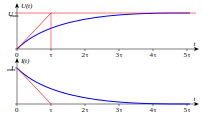
\includegraphics[width=\textwidth,keepaspectratio=true]{Ladevorgang.png}
      % Ladevorgang.png: 767x431 px, 96dpi, 20.30x11.41 cm, bb=0 0 575 323
      \caption{Von Honina.Frank Murmann at de:Wp via Wikipedia (abgerufen: 06.01.26)}
      \label{abb:CLadevorgang}
      \end{figure}
    \end{column}
  \end{columns}
\end{frame}

\begin{frame}{Aufladen eines Kondensators}
  \framesubtitle{Zeit bestimmen}
  gesucht: t
  \begin{align}
    u_c(t) &= U_0 \cdot (1- e^{-\frac{t}{\tau}})| : U_0\\
    \frac{u_c(t)}{U_0} &= 1- e^{-\frac{t}{\tau}}|-1, \cdot \ (-1) \\
    1-\frac{u_c(t)}{U_0} &= e^{-\frac{t}{\tau}}| ln()\\
    ln\left(1-\frac{u_c(t)}{U_0}\right) &= -\frac{t}{\tau}|\ \dot \  (-\tau)\\
    - \tau \cdot ln\left(1-\frac{u_c(t)}{U_0}\right) &= t
  \end{align}
   $\tau = R\cdot C,\ ln(x)$ ist Umkehrfunktion zu $e^x$
\end{frame}

\begin{frame}{Aufgaben - Laden des Kondensators}
\begin{tabular}{|l|l|l|l|l|l|}
  \hline
 $U_0$  & $U_c$    & $\tau$    & t &            R &  C\\ \hline
 12\, V & $U_c(t)$ &           & 100\ ms, 220\ ms, $3\tau$, 1\,s  & $1\ k\Omega$ & $220\ \mu F$\\ \hline
 12\, V & $U_c(t)$ & 0,484\, s & $2\tau$, 2\, s, 4\,s  &  & $220\ \mu F$\\ \hline
 12\, V & $U_c(t)$ & 1,034\, s & $0,5\tau$, $\tau$, 4\, s & $2,2\ k\Omega$ & \\ \hline
        & 8,56\, V & & 600 ms & $1,2\ k\Omega$ & $560 \mu F$ \\ \hline
\end{tabular}
\begin{itemize}
  \item berechnen die fehlenden Parameter($\tau$, R, C, $U_0$) und $U_C(t)$
 \item Bei Widerstandswerten und Kondensatorwerten sind jeweils Werte der E12-Reihe zu bestimmen.
 \item $U_c(t)$ = berechne alle Spannungen für $U_c$ zu den angegebenen Zeitpunkten t.
 \item Als weitere Übungsmöglichkeit: $U_0$ = 15\, V; 18\, V; 20\, V; 24\, V.
\end{itemize}
\end{frame}

\subsection{Kondensator entladen}
\begin{frame}{Entladen des Kondensators}
 \begin{itemize}
   \item Spannung fällt von $U_{max}$ auf 0\,V
   \item Strom fließt "`umgekehrt"'
   \item nach 5$\tau$ gilt der Kondensator als entladen.
 \end{itemize}
 \begin{align}
   u_c(t) &= U_0\cdot e^{-\frac{t}{\tau}}\\
   i_c(t) &= -\frac{U_0}{R}\cdot e^{-\frac{t}{\tau}}
 \end{align}
\end{frame}

\begin{frame}{Aufgaben: Laden und Entladen des Kondensators}
    \begin{columns}
      \begin{column}{.5\textwidth}
        \begin{figure}[htb]
        \begin{tikzpicture}
          \draw (0,0) to[vsource, l=$U_{0}$] (0,4) -- (2,4);
          \draw (2,4) to[opening switch, l={t = $t_1$}] (4,4) -- (5,4) -- (5,3);
          \draw (2,3) to[closing switch, l={t = $t_2$}] (4,3) --(5,3);
          \draw (5,3) node[circ]{} to (5,2.5);
          \draw (5,2.5) to [R=$R_1$] (5,1) to [C=$C_1$](5,0) -- (0,0);
          \draw (2,3) to[R=$R_2$] (2,0);
          \draw (2,0) node[circ]{};% to (5,2.5);
        \end{tikzpicture}
        \caption{Kondensator laden und entladen}
        \label{fig:StromkreisCLadenEntladen1}
      \end{figure}
    \end{column}
    \begin{column}{0.6\textwidth}
    \begin{tabular}{|l|l|l|l|l|}
      \hline
     $\tau 1$& $\tau 2$ & $R_1$& $R_2$& $C_1$\\ \hline
     &  & $1\, k\Omega$& $1,2\, k\Omega$& $100\mu F$\\ \hline
     &  & $3,3\, k\Omega$& $15\, k\Omega$& $220\mu F$\\ \hline
     &  & $47\, k\Omega$& $1\, k\Omega$& $470\mu F$\\ \hline
    \end{tabular}

    $U_0 = 12\,V$

    \begin{itemize}
     \item berechne $\tau$ für Ladung und Entladung
     \item welche Spannung hat der Kondensator nach 0,3s, 0,5s, 5s, 10 s?
     \item Wie lange dauert es, bis $3\tau$ erreicht sind?
     \item Wie groß muss $R_2$ sein, damit die Entladezeit um den Faktor 0,75; 1,5; 2; 2,5; 3 verändert wird?
    \end{itemize}
    \end{column}
  \end{columns}
\end{frame}

\begin{frame}{Beispiel: C laden "`ohne"' Vorwiderstand}
 Wie groß ist i(0+ = 1 ms), wenn folgendes gegeben ist:
 \begin{itemize}
  \item ideale Spannungsquelle (liefert definierte Spannung und "`beliebigen"' Strom).
  \item R = $1\ m\Omega$
  \item C = $10\mu \text{F}$
  \pause
  \item $\tau = R\cdot C$
  \item $\tau = 1\cdot 10^{-9}s$
  \pause
  \item $i_c(t) = -\frac{U_0}{R}\cdot e^{-\frac{t}{\tau}}$
  \item $i_c(t) = -\frac{5\, V}{1\ m\Omega}\cdot e^{-\frac{1\ ms}{1\  ns}}$
  \pause
  \item $i_c (t= 1\, ms) \approx 5\ kA$
 \end{itemize}
\end{frame}
! Nicht ausprobieren!\\
Ein Strom von ca. 5\,kA würde das Netzteil und die Schaltung (inklusive des Kondensators) zerstören. Bei einem Vorwiderstand von 0 steigt der Strom direkt nach dem Einschalten (wenige Pico Sekunden) theoretisch ins Unendliche. In Realität würden weder die Leiterbahn(en) noch die beteiligten Bauteile diese Stoßbelastung überstehen. Zusätzlich würden diverse andere Effekte auftreten, die hier aus Gründen der Vereinfachung ignoriert werden sollen.

\clearpage

\section[Magnete]{magnetisches Feld}
\begin{frame}{Beispiele Magnetfeld}
 \begin{itemize}
  \item Erdmagnetfeld
  \item Leitung (Strom durch flossen)
  \item Funk
  \item Spule, Motor(-wicklungen)
 \end{itemize}
\end{frame}

\subsection{magnetische Pole}
\begin{frame}{magnetische Pole}
 \begin{itemize}
  \item magnetische Feldlinien haben Anfang und Ende.
  \item Nordpol, Südpol
  \item Bei Dauermagnet, elektrischem Magnetfeld
 \end{itemize}
\end{frame}

\subsection{Unterschiede zum elektrischen Feld}
\begin{frame}{Unterschiede zum elektrischen Feld}
  \begin{description}
   \item[Elektrisches Feld] geschlossene Linien
   \item[Magnetisches Feld] Nordpol und Südpol
   \item[bei Elektrischem Strom] Magnetfeld steht senkrecht auf elektrischem Feld.
  \end{description}
\end{frame}

\subsection{Feldlinienbilder}
\begin{frame}{Feldlinien}
  \begin{columns}[c]
    \begin{column}{.5\textwidth }
      \begin{figure}
        \includegraphics{radar_out_v1_2_nurTopCuAusschnitt.png}
        % radar_out_v1_2_nurTopCuAusschnitt.png: 115x221 px, 300dpi, 0.97x1.87 cm, bb=0 0 28 53
        \caption{Leiterbahn auf Platine 12 V (Versorgung)}
        \label{abb:Leiterbahn1}
      \end{figure}
      \begin{figure}
        \includegraphics%[scale=2]
        {radar_out_v1_2_nurTopCuAusschnitt2.png}
        % radar_out_v1_2_nurTopCuAusschnitt2.png: 119x187 px, 300dpi, 1.01x1.58 cm, bb=0 0 29 45
        \caption{Leiterbahnen auf Platine (Relais-Ausgänge)}
        \label{abb:LeiterbahnAufPlatine2}
      \end{figure}
   \end{column}
    \begin{column}{.5\textwidth }
    \begin{description}
      \item[E-Feld] senkrecht, parallel zu Leiterbahn
      \item[Magnetfeld] senkrecht zur sichtbaren Ebene.
      \item[Massepotential] Gitter ist GND
    \end{description}
   \end{column}
  \end{columns}
\end{frame}

\begin{frame}{Überlagerung von Magnetfeldern}
  \begin{columns}
    \begin{column}{.3\textwidth}
     \includegraphics[scale=3]
        {radar_out_v1_2_nurTopCuAusschnitt2.png}
        % radar_out_v1_2_nurTopCuAusschnitt2.png: 119x187 px, 300dpi, 1.01x1.58 cm, bb=0 0 29 45
   \end{column}
    \begin{column}{.7\textwidth}
    \begin{itemize}
     \item Senkrechte Linie = Leiterbahn
     \item Gitter ist GND (Masse)
     \item Magnetfelder überlagern sich
     \item Induktion durch magnetisches Feld anderer Leiterbahnen
    \end{itemize}
   \end{column}
  \end{columns}
\end{frame}
\subsection{Formen von Magneten}
\begin{frame}{Formen von Magneten}
  \begin{itemize}
  \item  Permanentmagnet
  \item Elektromagnet
  \end{itemize}
\end{frame}

\subsection{Magnetische Kraftwirkung (LORENTZ-Kraft, Selbstinduktion)}

\section[noch offen]{Pflicht-Themen, die noch offen sind}
\begin{frame}{Pflicht-Themen, die noch offen sind}
Folgende Themen sind gemäß Prüfungserlass für die Prüfung 2026 Pflicht, aber noch nicht ausgearbeitet.
  \begin{itemize}
%     \item Kondensator
%     \\ Auf- und Entladung
    \item Induktion
    \\ Magnetischer Fluss (Phi)
    \\ Flussdichte (B)
    \item Spule
    \\ Ein- und Ausschaltvorgang
  \end{itemize}

  Die Themen folgen demnächst hier.
\end{frame}

\appendix
\section{Lösungsvorschläge zu Aufgaben}
\begin{frame}
  \centering{\Huge{Anhang}}
\end{frame}


\begin{frame}{Zu Folie \ref{KraftAufLadungAufgabe1}}

\begin{columns}
\column{.4\textwidth}
\begin{figure}[h]
  \begin{tikzpicture}
      \draw[step=.5 cm, gray!50, very thin] (0,0) grid (4,3);
      \draw[->] (-.5,0) -- (5,0);
      \draw[->] (0,-.5) -- (0,4);
      %\draw node[circ] at (0,0){};
      \filldraw[white] (1,1) circle [radius=5pt]
                 (3,1) circle [radius=5pt]
                 (2,2) circle [radius=5pt];
      \draw (1,1) circle [radius=5pt]
                 (3,1) circle [radius=5pt]
                 (2,2) circle [radius=5pt];
      \draw node at (1,1) {+};
      \draw node at (2,2) {+};
      \draw node at (3,.95) {-};
      \draw node at (0.5,1) {$Q_1$};
      \draw node at (2.5,1) {$Q_2$};
      \draw node at (1.5,2) {$Q_3$};
      \draw[<->] (1.2,1.2) -- (1.8,1.8);
      \draw[>-<] (2.8,1.2) -- (2.2,1.8);
  \end{tikzpicture}
\end{figure}

\column{.6\textwidth}
$F_{31} = \frac{Q_1\cdot Q_2}{4\cdot \pi \cdot \varepsilon_0 \cdot r^2}$\\
$F_{31} = \frac{10\mu C^2}{4\cdot \pi \cdot \varepsilon_0 \cdot \sqrt{2}m^2}$\\
$F_{31} = \frac{10\mu As^2}{4\cdot \pi \cdot 8,85*10^{-12}\frac{As}{Vm} \cdot \sqrt{2}m^2}$\\

  $|F_{31}| = 0,64 N$. Da $Q_1, Q_2 \ \text{und} \ Q_3$ gleich groß sind und der Abstand ebenfalls gleich ist, ist $F_{32} = 0,64 N$
$|F_{31}| = 0,64 N$. Da $Q_1, Q_2 \ \text{und} \ Q_3$ gleich groß sind und der Abstand ebenfalls gleich ist, ist $F_{32} = 0,64 N$
\end{columns}
\end{frame}

\begin{frame}{zu Folie\ref{AufgabeUeberlagerungE-Felder}}
\begin{columns}
\column{.4\textwidth}
\begin{figure}[h]
  \begin{tikzpicture}
      \draw[step=.5 cm, gray!50, very thin] (0,0) grid (4,3);
      \draw[->] (-.5,0) -- (5,0);
      \draw[->] (0,-.5) -- (0,4);
      %\draw node[circ] at (0,0){};
      \filldraw[white] (1,1) circle [radius=5pt]
                 (3,1) circle [radius=5pt]
                 (2,1) circle [radius=5pt];
%                  (2,2) circle [radius=5pt];
      \draw (1,1) circle [radius=5pt]
                 (3,1) circle [radius=5pt]
                 (2,1) circle [radius=5pt];
%                  (2,2) circle [radius=5pt];
      \draw node at (1,1) {+};
      \draw node at (3,.95) {-};
      \draw node at (1,0.5) {$Q_1$};
      \draw node at (3,0.5) {$Q_2$};
      \draw node at (2,0.5) {$P_1$};
%       \draw node at (1.5,2) {$P_n$};
      \draw[->] (1.2,1) -- (1.8,1);
      \draw[->] (2.8,1) -- (2.2,1);
  \end{tikzpicture}
\end{figure}

  \column{.6\textwidth}
  Abstand $Q_1 - P_1: P_1 - Q_1 = $
  $\left( \begin{array}{c}1\,m \\ 0\, m\end{array} \right) - \left( \begin{array}{c}0\,m \\ 0\, m\end{array} \right) = \sqrt{1\,m^2 + 0\, m^2} = 1\,m$%\\
  \begin{align*}
    E &= \frac{Q}{4 \cdot \pi \cdot r^2 \cdot \varepsilon}\\
    E_{p1_{q1}} &= \frac{Q_1}{4 \cdot \pi \cdot r^2 \cdot \varepsilon_0}\\
    E_{p1_{q1}} &= \frac{3\ nC}{4 \cdot \pi \cdot 1\,m^2 \cdot \varepsilon_0}\\
    E_{p1_{q1}} &= \frac{3\ nAs}{4 \cdot \pi \cdot 1\,m^2 \cdot 8,85\cdot10^{-12}\frac{As}{Vm}}\\E_{p1_{q1}} &= 26,9\ \frac{V}{m}
  \end{align*}
\end{columns}
\end{frame}


\begin{frame}
 \begin{align*}
    E &= \frac{Q}{4 \cdot \pi \cdot r^2 \cdot \varepsilon}\\
    E_{p1_{q2}} &= \frac{Q_1}{4 \cdot \pi \cdot r^2 \cdot \varepsilon_0}\\
    E_{p1_{q2}} &= \frac{-10\ nC}{4 \cdot \pi \cdot 1\,m^2 \cdot \varepsilon_0}\\
    E_{p1_{q1}} &= \frac{-10\ nAs}{4 \cdot \pi \cdot 1\,m^2 \cdot 8,85\cdot10^{-12}\frac{As}{Vm}}\\
    E_{p1_{q2}} &= -98,82\ \frac{V}{m}\\
    E_{p1} &= 26,9\frac{V}{m} -98,82\ \frac{V}{m} = 62,92\frac{V}{m}
  \end{align*}
\end{frame}


\begin{frame}{zu Folie\ref{AufgabeUeberlagerungE-Felder}, Abstand der Punkte zur Ladung}
\begin{columns}
\column{.4\textwidth}
\begin{figure}[h]
  \begin{tikzpicture}
      \draw[step=.5 cm, gray!50, very thin] (0,0) grid (4,3);
      \draw[->] (-.5,1) -- (5,1);
      \draw[->] (1,-.5) -- (1,4);
      %\draw node[circ] at (0,0){};
      \filldraw[white] (1,1) circle [radius=5pt]
                 (3,1) circle [radius=5pt]
                 (2,1) circle [radius=5pt]
                 (1.5,1.5) circle [radius=5pt]
                 (1.5,1) circle [radius=5pt]
                 (2,2) circle [radius=5pt];
      \draw (1,1) circle [radius=5pt]
                 (3,1) circle [radius=5pt]
                 (2,1) circle [radius=5pt]
                 (1.5,1.5) circle [radius=5pt]
                 (1.5,1) circle [radius=5pt]
                 (2,2) circle [radius=5pt];
      \draw node at (1,1) {+};
      \draw node at (3,.95) {-};
      \draw node at (.7,0.5) {$Q_1$};
      \draw node at (3,0.5) {$Q_2$};
      \draw node at (2,1) {1};
      \draw node at (3.5,0.5) {$P_2$};
      \draw node at (1.5,1.5) {3};
      \draw node at (1.5,1) {4};
      \draw node at (2,2) {5};
%       \draw node at (1.5,2) {$P_n$};
%       \draw[->] (1.2,1) -- (1.8,1);
%       \draw[->] (2.8,1) -- (2.2,1);
  \end{tikzpicture}
\end{figure}
\end{columns}
\end{frame}

\begin{frame}{zu Folie\ref{AufgabeUeberlagerungE-Felder}, Abstand der Punkte zur Ladung}
\begin{columns}
\column{.4\textwidth}
\begin{figure}[h]
  \begin{tikzpicture}
      \draw[step=.5 cm, gray!50, very thin] (0,0) grid (4,3);
      \draw[->] (-.5,1) -- (5,1);
      \draw[->] (1,-.5) -- (1,4);
      %\draw node[circ] at (0,0){};
      \filldraw[white] (1,1) circle [radius=5pt]
                 (3,1) circle [radius=5pt]
%                  (2,1) circle [radius=5pt]
                 (1.5,1.5) circle [radius=5pt]
%                  (1.5,1) circle [radius=5pt]
%                  (2,2) circle [radius=5pt]
;
      \draw (1,1) circle [radius=5pt]
                 (3,1) circle [radius=5pt]
%                  (2,1) circle [radius=5pt]
                 (1.5,1.5) circle [radius=5pt]
%                  (1.5,1) circle [radius=5pt]
%                  (2,2) circle [radius=5pt]
;
      \draw node at (1,1) {+};
      \draw node at (3,.95) {-};
      \draw node at (.7,0.5) {$Q_1$};
      \draw node at (3,0.5) {$Q_2$};
%       \draw node at (2,1) {1};
%       \draw node at (3.5,0.5) {$P_2$};
      \draw node at (1.5,1.5) {3};
%       \draw node at (1.5,1) {4};
%       \draw node at (2,2) {5};
%       \draw node at (1.5,2) {$P_n$};
      \draw[->] (1.2,1.2) -- (1.3,1.3);
      \draw[->] (2.8,1.1) -- (1.7,1.43);
  \end{tikzpicture}
\end{figure}
\end{columns}
\end{frame}
\clearpage
\subsection{Kondensator}
\begin{frame}{Aufgaben - Laden des Kondensators}
  \subtitle{Lösungen}
  \label{AufgabenLadenC-Lsg}
\begin{tabular}{|l|l|l|l|l|l|}
 $U_0$  & $U_c$    & $\tau$    & t &            R &  C\\ \hline
 12\, V & \underline{siehe unten} & \underline{0,22\, s}  & 100\ ms, 220\ ms, $3\tau$, 1\,s  & $1\ k\Omega$ & $220\ \mu F$\\
 12\, V & $U_c(t)$ & 0,484\, s & $2\tau$, 2\, s, 4\,s  & \underline{$2,2k\Omega$} & $220\ \mu F$\\
 12\, V & $U_c(t)$ & 1,034\, s & $0,5\tau$, $\tau$, 4\, s & $2,2\ k\Omega$ & \underline{$470\ \mu F$} \\
 \underline{14,5\, V}& 8,56\, V & \underline{0,672\, s}& 600 ms & $1,2\ k\Omega$ & $560 \mu F$ \\
\end{tabular}
\end{frame}
\begin{frame}{Aufgaben Laden C LSG Teil 2}
  \begin{columns}[t]
    \begin{column}{.5\textwidth}
    Zu Zeile 1 (12V, $\tau = 0,22 s$, R = $1\, k\Omega$, C~=~$220\ \mu F$)

\begin{tabular}{|l|l|}
  \hline
 t & $U_c(t)$ \\ \hline
 100 ms & 4,38\, V \\ \hline
 220 ms & 7,59\, V \\ \hline
 $3\tau$ = 0,66 s & 11,4\, V\\ \hline
 1\, s & 11,9V\\ \hline
\end{tabular}

Zu Zeile 2 (12V, $\tau = 0,484 s$, R~=~$2,2\, k\Omega$, C = $220\ \mu F$)

\begin{tabular}{|l|l|}
  \hline
 t & $U_c(t)$ \\ \hline
 $2\tau = 0,968 s$ & 10,4\, V \\ \hline
 2\, s & 11,8\, V \\ \hline
 4\, s & 12,0\,V\\ \hline
\end{tabular}
    \end{column}
    \begin{column}{.5\textwidth}

    Zu Zeile 3 (12V, $\tau = 1,034 s$, R~=~$2,2\, k\Omega$, C = $470\ \mu F$)

\begin{tabular}{|l|l|}
  \hline
 t & $U_c(t)$ \\ \hline
 $0,5\tau = 0,517 s$ & 4,72\, V \\ \hline
 $\tau = 0,672\, s$ & 7,58\, V \\ \hline
 4\, s & 11,97\,V\\ \hline
\end{tabular}
    \end{column}
  \end{columns}
\end{frame}




% \begin{figure}[h]
%   \begin{tikzpicture}
%
% \draw[x=1ex,y=1ex] (0,0) sin (1,1) cos (2,0) sin (3,-1) cos (4,0)
% (0,1) cos (1,0) sin (2,-1) cos (3,0) sin (4,1);
%   \end{tikzpicture}
% \end{figure}
